%%%%%%%%%%%%%%%%%%%%%%%%%%%%%%%%%%%%%%%%%%%%%%%%%%%%%%%%%%%%%%%%%%%%%%
% Ejemplo de Informe de Práctica Profesional II
%%%%%%%%%%%%%%%%%%%%%%%%%%%%%%%%%%%%%%%%%%%%%%%%%%%%%%%%%%%%%%%%%%%%%%
\documentclass[12pt,a4paper]{report}

% Codificación e idioma
\usepackage[utf8]{inputenc}
\usepackage[T1]{fontenc}
\usepackage[spanish]{babel}

% Selección de fuente: se usa newtxtext para apariencia similar a Times New Roman.
\usepackage{newtxtext,newtxmath}

% Paquetes gráficos y de geometría
\usepackage{graphicx}
\usepackage{geometry}
\geometry{margin=2.5cm}

% Paquetes para cabecera y pie de página
\usepackage{fancyhdr}
\pagestyle{fancy}
\renewcommand{\headrulewidth}{1pt} % Línea inferior en el encabezado

% Definir encabezado y pie de página
\fancyhead{} % Limpiar encabezados
\fancyhead[L]{\textbf{Práctica Profesional II}} % Encabezado a la izquierda
\fancyfoot{} % Limpiar pie de página
\fancyfoot[L]{Álvaro Iván Loyola Mendoza - 21.151.773-5} % Pie de página a la izquierda
\fancyfoot[R]{\thepage} % Número de página a la derecha

% Redefinir el estilo "plain" para que utilice la misma configuración que "fancy"
\fancypagestyle{plain}{
  \fancyhf{}
  \fancyhead[L]{\textbf{Práctica Profesional II}}
  \fancyfoot[L]{Álvaro Iván Loyola Mendoza - 21.151.773-5}
  \fancyfoot[R]{\thepage}
  \renewcommand{\headrulewidth}{1pt}
}

\usepackage[table]{xcolor} % Para colores en tablas
\usepackage{array} % Para mejorar alineación en tablas
\usepackage{longtable} % Para tablas largas si es necesario
\usepackage{multirow} % Para fusionar filas
\usepackage{booktabs} % Para mejores líneas en la tabla

% Paquete para modificar formato de títulos (titlesec)
\usepackage{titlesec}
% Ajustar el formato de capítulo: se reduce el espacio superior y se ajusta el tamaño del título
\titleformat{\chapter}[hang]{\LARGE\bfseries}{\thechapter.}{1em}{}
\titlespacing*{\chapter}{0pt}{-20pt}{20pt} % Ajuste: disminuye el espacio superior a los capítulos

% Espaciado entre párrafos y sin sangría
\setlength{\parskip}{\baselineskip}
\setlength{\parindent}{0pt}
\linespread{1} % Interlineado simple

% Paquetes para tablas y figuras (opcional, para índices si hay contenido)
\usepackage{caption}
\usepackage{float}

% Paquete para bibliografía en formato APA (puede ajustarse o usar apacite, biblatex, etc.)
\usepackage{apacite}
\bibliographystyle{apacite}
\usepackage{hyperref}

\begin{document}

% Asegurarse de que el resto de las páginas usen el estilo fancy
\pagestyle{fancy}

%%%%%%%%%%%%%%%%%%%%%%%%%%%%%%%%%%%%%%%%%%%%%%
% PORTADA
%%%%%%%%%%%%%%%%%%%%%%%%%%%%%%%%%%%%%%%%%%%%%%
\begin{titlepage}
    \thispagestyle{empty} % No mostrar encabezado ni pie en la portada
    \centering
    % Inserte el logo de la Universidad (coloque el archivo en la misma carpeta o especifique la ruta)
    
\includegraphics[width=12cm]{images/logo-universidad.png}\par
    \vspace{1cm}
    {\huge\bfseries Práctica Profesional II\\[0.5em]620456 - 1\par}
    \vspace{1cm}
    {\Large Nombre Estudiante: Álvaro Iván Loyola Mendoza\par}
    {\Large Profesor Supervisor: Ariel Alfredo Andia Roa\par}
    {\Large Fecha: 01 de marzo de 2025\par}
    \vfill
\end{titlepage}
% Forzamos que la numeración inicie en 1, contabilizando la portada como página 1.
\setcounter{page}{2}



%%%%%%%%%%%%%%%%%%%%%%%%%%%%%%%%%%%%%%%%%%%%%%
% ÍNDICES
%%%%%%%%%%%%%%%%%%%%%%%%%%%%%%%%%%%%%%%%%%%%%%
\tableofcontents
\newpage
\listoffigures
\newpage

%%%%%%%%%%%%%%%%%%%%%%%%%%%%%%%%%%%%%%%%%%%%%%
% CAPÍTULO: Introducción
%%%%%%%%%%%%%%%%%%%%%%%%%%%%%%%%%%%%%%%%%%%%%%
\chapter{Introducción}
La práctica profesional es una instancia clave en la formación de un ingeniero en informática, ya que permite la aplicación de conocimientos teóricos en un entorno real de trabajo. En este contexto, la presente práctica se llevó a cabo en Factoring Security, una empresa del sector financiero dedicada a la gestión de factoring y financiamiento, específicamente en el área de Quality Assurance (QA) dentro de proyectos de tecnología.

El objetivo principal de esta práctica fue adquirir experiencia en la ejecución de pruebas de software dentro del proceso de aseguramiento de calidad, garantizando que las soluciones tecnológicas desarrolladas en la empresa cumplan con los estándares requeridos antes de su implementación. Para ello, se participó activamente en el equipo de QA, encargado de evaluar la calidad de los desarrollos en el proyecto de cambio de core, un proceso crítico para la organización.

Durante el período comprendido entre el 6 de enero y el 28 de febrero de 2025, se llevaron a cabo diversas actividades, entre las que destacan la ejecución sistemática de pruebas de sistemas, la documentación detallada de hallazgos y defectos, el reporte de incidencias al equipo de desarrollo, la realización de pruebas de regresión para validar nuevas funcionalidades y la entrega de avances periódicos, con el fin de garantizar un flujo eficiente en el proceso de control de calidad.

A través de esta experiencia, no solo se profundizó en la práctica del testing de software y la identificación de errores, sino que también se desarrollaron habilidades fundamentales en trabajo en equipo, comunicación efectiva y resolución de problemas dentro de un ambiente profesional. Este informe detalla el contexto de la empresa, las actividades realizadas, los resultados obtenidos y las conclusiones derivadas de la práctica, proporcionando una visión integral de los aprendizajes adquiridos.

%%%%%%%%%%%%%%%%%%%%%%%%%%%%%%%%%%%%%%%%%%%%%%
% CAPÍTULO: Desarrollo de la Práctica
%%%%%%%%%%%%%%%%%%%%%%%%%%%%%%%%%%%%%%%%%%%%%%
\chapter{Desarrollo de la Práctica}

%%%%%%%%%%%%%%%%%%%%%%%%%%%%%%%%%%%%%%%%%%%%%%
% Sección: Descripción del Centro de Práctica
%%%%%%%%%%%%%%%%%%%%%%%%%%%%%%%%%%%%%%%%%%%%%%
\section{Descripción del Centro de Práctica}
Factoring Security S.A. es una empresa filial del Grupo Security, nace en 1992 para otorgar soluciones a los problemas de liquidez, cobranza, administración y financiamiento de sus clientes en forma ágil y oportuna.
\begin{itemize}
    \item \textbf{Nombre o Razón Social:} Factoring Security S.A.
    \item \textbf{RUT:} 96.655.860-1
    \item \textbf{Representante Legal:} Ignacio Prado R. RUT: 7.106.815-3
    \item \textbf{Dirección Postal:} Av. Apoquindo 3150, Las Condes, Santiago.
    \item \textbf{Sitio Web:} https://www.factoringsecurity.cl/
    \item \textbf{Teléfono:} (41) 290 8050
    \item \textbf{Área de Práctica:} Quality Assurance (QA)
    \item \textbf{Organigrama:} \begin{figure}[H]
      \centering
      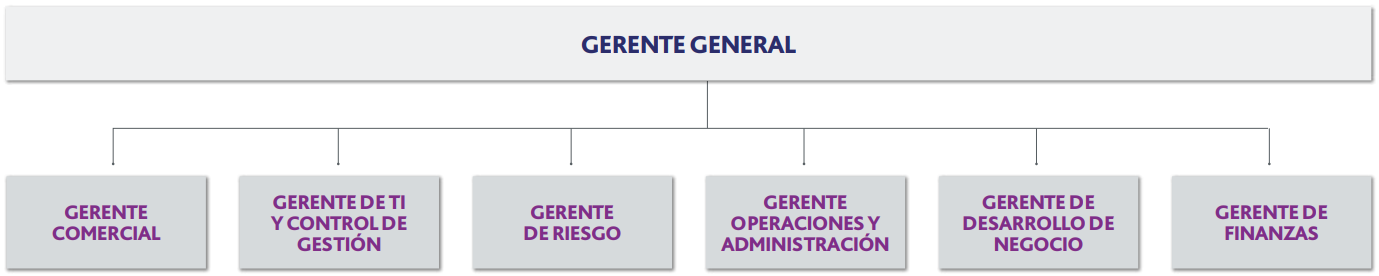
\includegraphics[width=14cm]{images/organigrama.png}
      \caption{Estructura Corporativa de Factoring Security}
    \end{figure}
    \item \textbf{Objetivos:}
    \begin{itemize}
        \item Brindar soluciones financieras flexibles y adaptadas a las necesidades de liquidez de las pequeñas y medianas empresas.
        \item Agilizar el proceso de aprobación de operaciones de factoring para garantizar una rápida disponibilidad de los recursos financieros.
        \item Mantener altos estándares de calidad en el servicio al cliente, ofreciendo atención personalizada y satisfaciendo las necesidades de cada empresa.
        \item Contribuir al crecimiento y desarrollo de las empresas a las que presta sus servicios, optimizando su flujo de caja y facilitando su operatividad.
        \item Consolidar su posición en el mercado como una empresa líder en el sector de factoring, basada en la confianza, la transparencia y la eficiencia en sus operaciones.
    \end{itemize}
    \item \textbf{Misión:} Nuestra misión es entregar un servicio de excelencia. Queremos exceder las expectativas de nuestros clientes, para lograr un reconocimiento, lealtad y recomendaciones favorables en el mercado. Queremos motivar y desarrollar a nuestros empleados logrando un sentido de pertenencia en un contexto que concilie Trabajo y Familia.
    \item \textbf{Visión:} Seremos la primera opción de Factoring en Chile, entregando un servicio ágil, flexible y eficiente, con soluciones integrales de liquidez y servicios de cobranza que garanticen altos niveles de fidelidad y satisfacción de nuestros clientes.
    \item \textbf{Valores:} Los valores de Factoring Security S.A. son los siguientes:
    \begin{itemize}
      \item \textbf{Transparencia:} Actuar con honestidad, integridad y claridad en todas las operaciones y relaciones comerciales.
      \item \textbf{Confianza:} Generar relaciones sólidas y duraderas con los clientes, basadas en la confianza mutua y el compromiso.
      \item \textbf{Excelencia:} Buscar la mejore continua en la calidad de los servicios y la satisfacción del cliente.
      \item \textbf{Respeto:} Valorar y respetar a todas las personas, clientes, colaboradores y socios comerciales.
      \item \textbf{Responsabilidad:} Cumplir con los compromisos adquiridos y actuar de manera ética y responsable en todas las actividades de la empresa.
      \item \textbf{Innovación:} Estar en constante búsqueda de nuevas soluciones y herramientas financieras para mejorar el servicio y adptarse a las necesidades del mercado.
      \item \textbf{Colaboración:} Fomentar el trabajo en equipo y la colaboración entre los diferentes departamentos de la empresa para lograr los objetivos comunes.
    \end{itemize}

\end{itemize}

\bigskip

%%%%%%%%%%%%%%%%%%%%%%%%%%%%%%%%%%%%%%%%%%%%%%
% Sección: Descripción de la Práctica
%%%%%%%%%%%%%%%%%%%%%%%%%%%%%%%%%%%%%%%%%%%%%%
\section{Descripción de la Práctica}

\subsection{Resumen General}

La práctica profesional se llevó a cabo en \textbf{Factoring Security}, una empresa del sector financiero enfocada en la gestión de factoring y financiamiento. La práctica se realizó en el área de \textbf{Quality Assurance (QA)} dentro del departamento de proyectos de tecnología, con el objetivo de adquirir experiencia en el proceso de aseguramiento de calidad de software.

El propósito principal fue participar activamente en la ejecución de pruebas para garantizar la calidad y el correcto funcionamiento de las soluciones tecnológicas en desarrollo. Se trabajó en el proyecto de cambio de core, un proceso clave dentro de la empresa, en el cual se verificó que las nuevas implementaciones cumplieran con los estándares de calidad antes de su despliegue.

Durante el período de práctica, se llevaron a cabo diversas actividades, tales como la ejecución de pruebas de sistemas, la documentación detallada de hallazgos, el reporte de defectos al equipo de desarrollo, la realización de pruebas de regresión y la entrega de avances periódicos sobre las actividades realizadas. Estas tareas permitieron no solo fortalecer habilidades técnicas relacionadas con el testing de software, sino también desarrollar competencias en comunicación, trabajo en equipo y resolución de problemas dentro de un entorno profesional.

\subsection{Actividades Realizadas}

A continuación, se describen las actividades realizadas durante la práctica, junto con sus respectivas características y resultados.

\begin{itemize}
    \item \textbf{Tareas Específicas:}
    \begin{itemize}
        \item \textbf{Ejecución de pruebas de sistemas:} Realización de pruebas funcionales para verificar el correcto desempeño de las aplicaciones, identificando posibles errores y fallos en las funcionalidades implementadas.
        \item \textbf{Documentación de hallazgos:} Registro detallado de los defectos detectados, incluyendo los pasos para su reproducción, el entorno en el que ocurrieron y su impacto en el sistema.
        \item \textbf{Reporte de defectos:} Comunicación de los problemas identificados al equipo de desarrollo a través de herramientas de gestión de errores, proporcionando información clara y precisa para su resolución.
        \item \textbf{Pruebas de regresión:} Validación de que los cambios realizados en el sistema no afectaran funcionalidades previamente implementadas, asegurando la estabilidad del software.
        \item \textbf{Entrega de reportes de avance:} Presentación periódica de informes de progreso, identificando riesgos y posibles dificultades en la ejecución de pruebas.
    \end{itemize}

    \item \textbf{Áreas Involucradas:}
    \begin{itemize}
        \item \textbf{Departamento de Tecnología:} Responsable del desarrollo, implementación y mantenimiento de soluciones tecnológicas dentro de la empresa.
        \item \textbf{Equipo de QA:} Encargado de velar por la calidad del software mediante la ejecución de pruebas y la validación de funcionalidades.
        \item \textbf{Equipo de Desarrollo (Externo):} Recibió los reportes de errores y trabajó en la corrección de defectos identificados durante la ejecución de pruebas.
    \end{itemize}

    \item \textbf{Herramientas y Plataformas Usadas:}
    \begin{itemize}
        \item \textbf{Microsoft Azure:} Utilizado para la gestión de backlogs, seguimiento de tareas y reporte de defectos en el desarrollo de software.
        \item \textbf{Microsoft SharePoint:} Plataforma utilizada para acceder a la documentación del proyecto, incluyendo guías, especificaciones técnicas y procedimientos internos.
        \item \textbf{Excel:} Empleado para el registro y organización de datos relacionados con las pruebas, así como para la sistematización de evidencias y reportes.
        \item \textbf{Notion:} Herramienta utilizada para coordinar la entrega de evidencias, documentar hallazgos y realizar seguimiento a los avances de la práctica.
    \end{itemize}

    \item \textbf{Resultados Obtenidos:}
    \begin{itemize}
        \item Identificación y documentación de errores que permitieron mejorar la estabilidad del software.
        \item Optimización del proceso de pruebas, reduciendo el tiempo de detección y corrección de fallos.
        \item Fortalecimiento de habilidades en análisis de calidad, documentación técnica y comunicación efectiva con el equipo de desarrollo.
    \end{itemize}
\end{itemize}

\subsection{Conclusiones de la Práctica}

La práctica profesional permitió adquirir experiencia real en el proceso de aseguramiento de calidad dentro del ámbito financiero y tecnológico. A través de la ejecución de pruebas y la documentación de hallazgos, se logró contribuir a la estabilidad y mejora del software en desarrollo.

Para la empresa, los beneficios fueron significativos, ya que la detección temprana de defectos redujo el impacto de errores en etapas avanzadas del desarrollo, optimizando tiempos y costos en la implementación de soluciones. Además, la documentación detallada de pruebas facilitó la trazabilidad de incidencias y permitió una gestión más eficiente de los problemas reportados.

Desde el punto de vista personal, esta experiencia permitió reforzar conocimientos en \textbf{pruebas de software, detección y documentación de defectos, y gestión de calidad} en entornos corporativos. También se fortalecieron habilidades transversales como \textbf{trabajo en equipo, comunicación efectiva y resolución de problemas}, aspectos fundamentales para el desarrollo profesional en el área de ingeniería en informática.

En conclusión, la práctica en \textbf{Factoring Security} representó una oportunidad valiosa para aplicar conocimientos adquiridos en la carrera y comprender de manera práctica la importancia del aseguramiento de calidad en proyectos tecnológicos dentro del sector financiero.
\bigskip

\subsection{Bibliografía}
Sobre Factoring Security | Factoring Security | Factoring Security. (n.d.). \url{https://www.factoringsecurity.cl/sobre-factoring-security}.

Preguntas frecuentes | Factoring Security. (n.d.). \url{https://www.factoringsecurity.cl/preguntas-frecuentes}.

Factoring Security. (2022). Memoria Integrada Factoring Security 2022. Recuperado de \url{https://www.factoringsecurity.cl/sites/factoring/files/reporte_integrado_factoring_security_2022.pdf}.

%%%%%%%%%%%%%%%%%%%%%%%%%%%%%%%%%%%%%%%%%%%%%%
% CAPÍTULO: Anexos
%%%%%%%%%%%%%%%%%%%%%%%%%%%%%%%%%%%%%%%%%%%%%%
\chapter{Anexos}
Se adjuntan las evidencias de las tareas realizadas, fotografías de la oficina, pantallas de los sistemas utilizados, manuales y documentos consultados, y bitácoras de actividades. Las imagenes borrosas son por motivos de privacidad, no se pueden mostrar datos sensibles de la empresa.
\begin{itemize}
    \item \textbf{Evidencias de las tareas realizadas:}
    \begin{figure}[H]
      \centering
      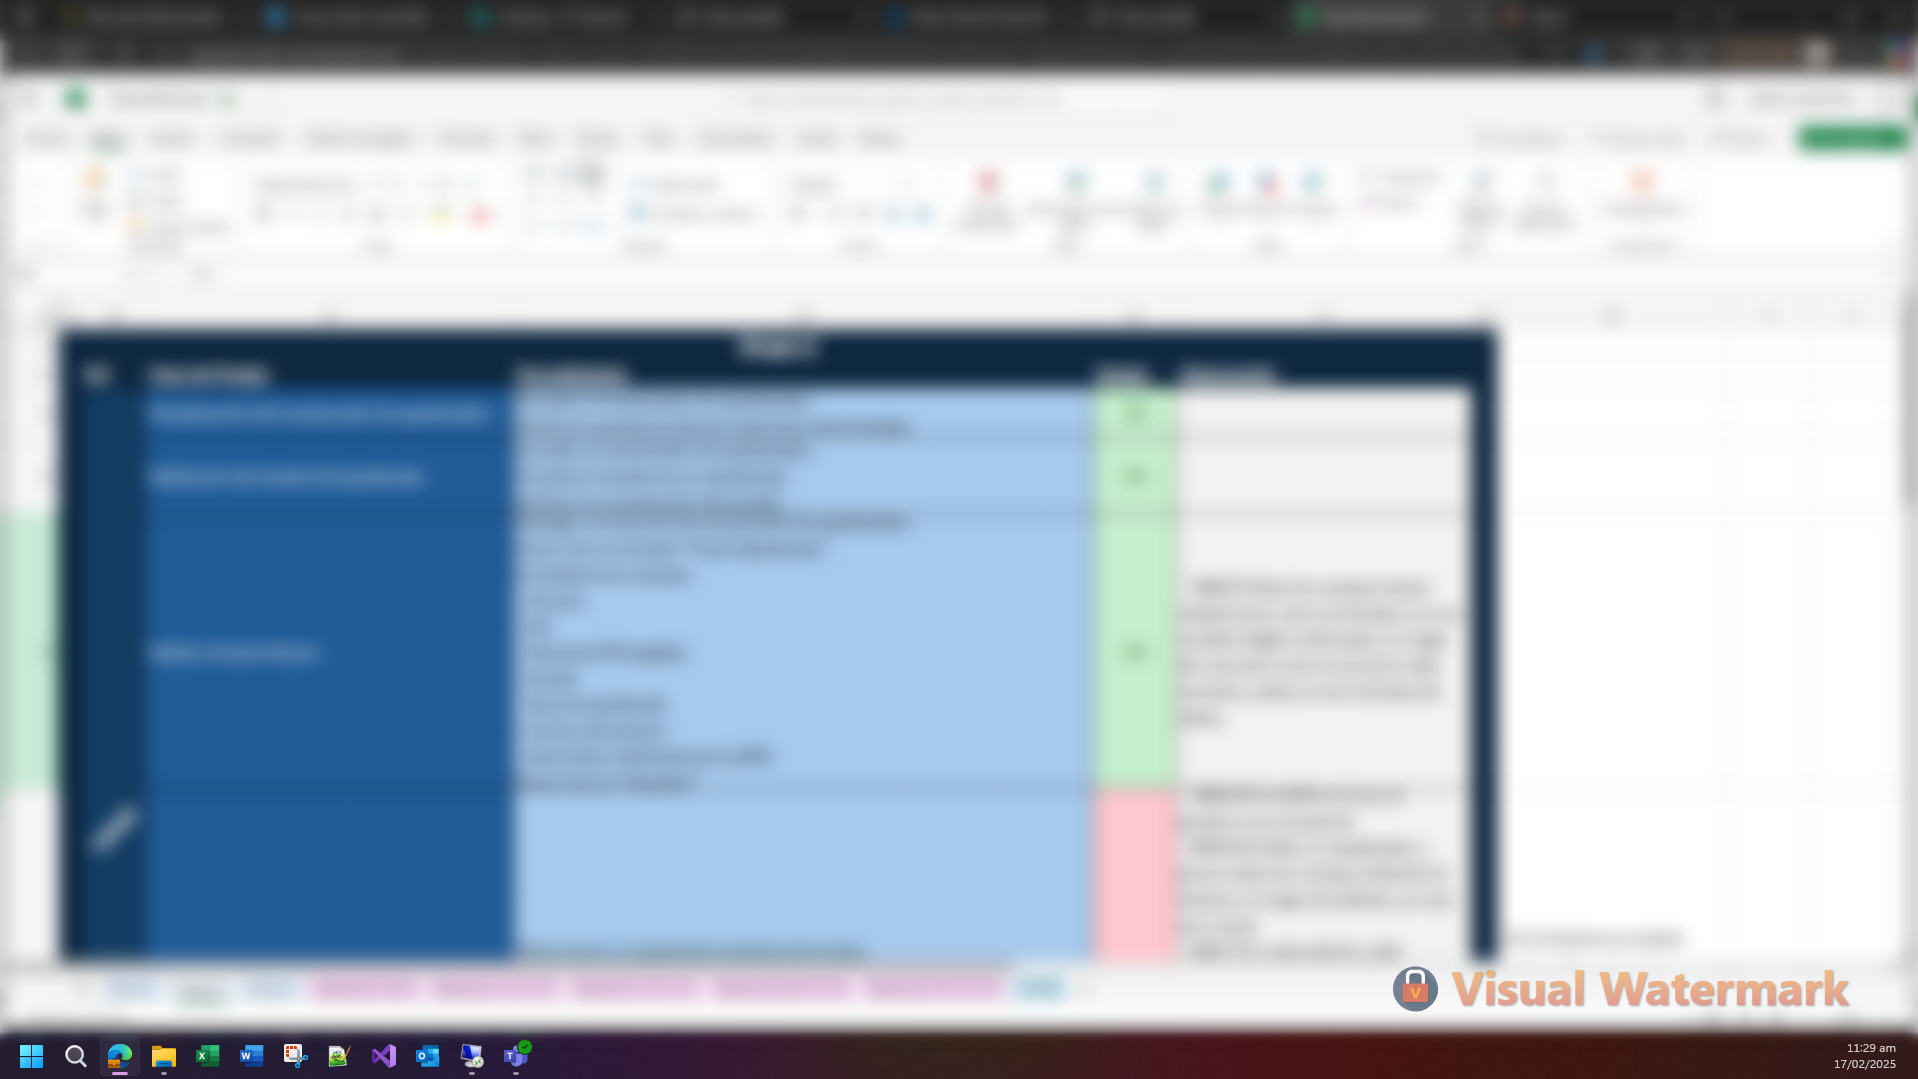
\includegraphics[width=14cm]{images/evidenciatareasrealizadas/excel.png}
      \caption{Registro de pruebas en Excel}
    \end{figure}
    \begin{figure}[H]
      \centering
      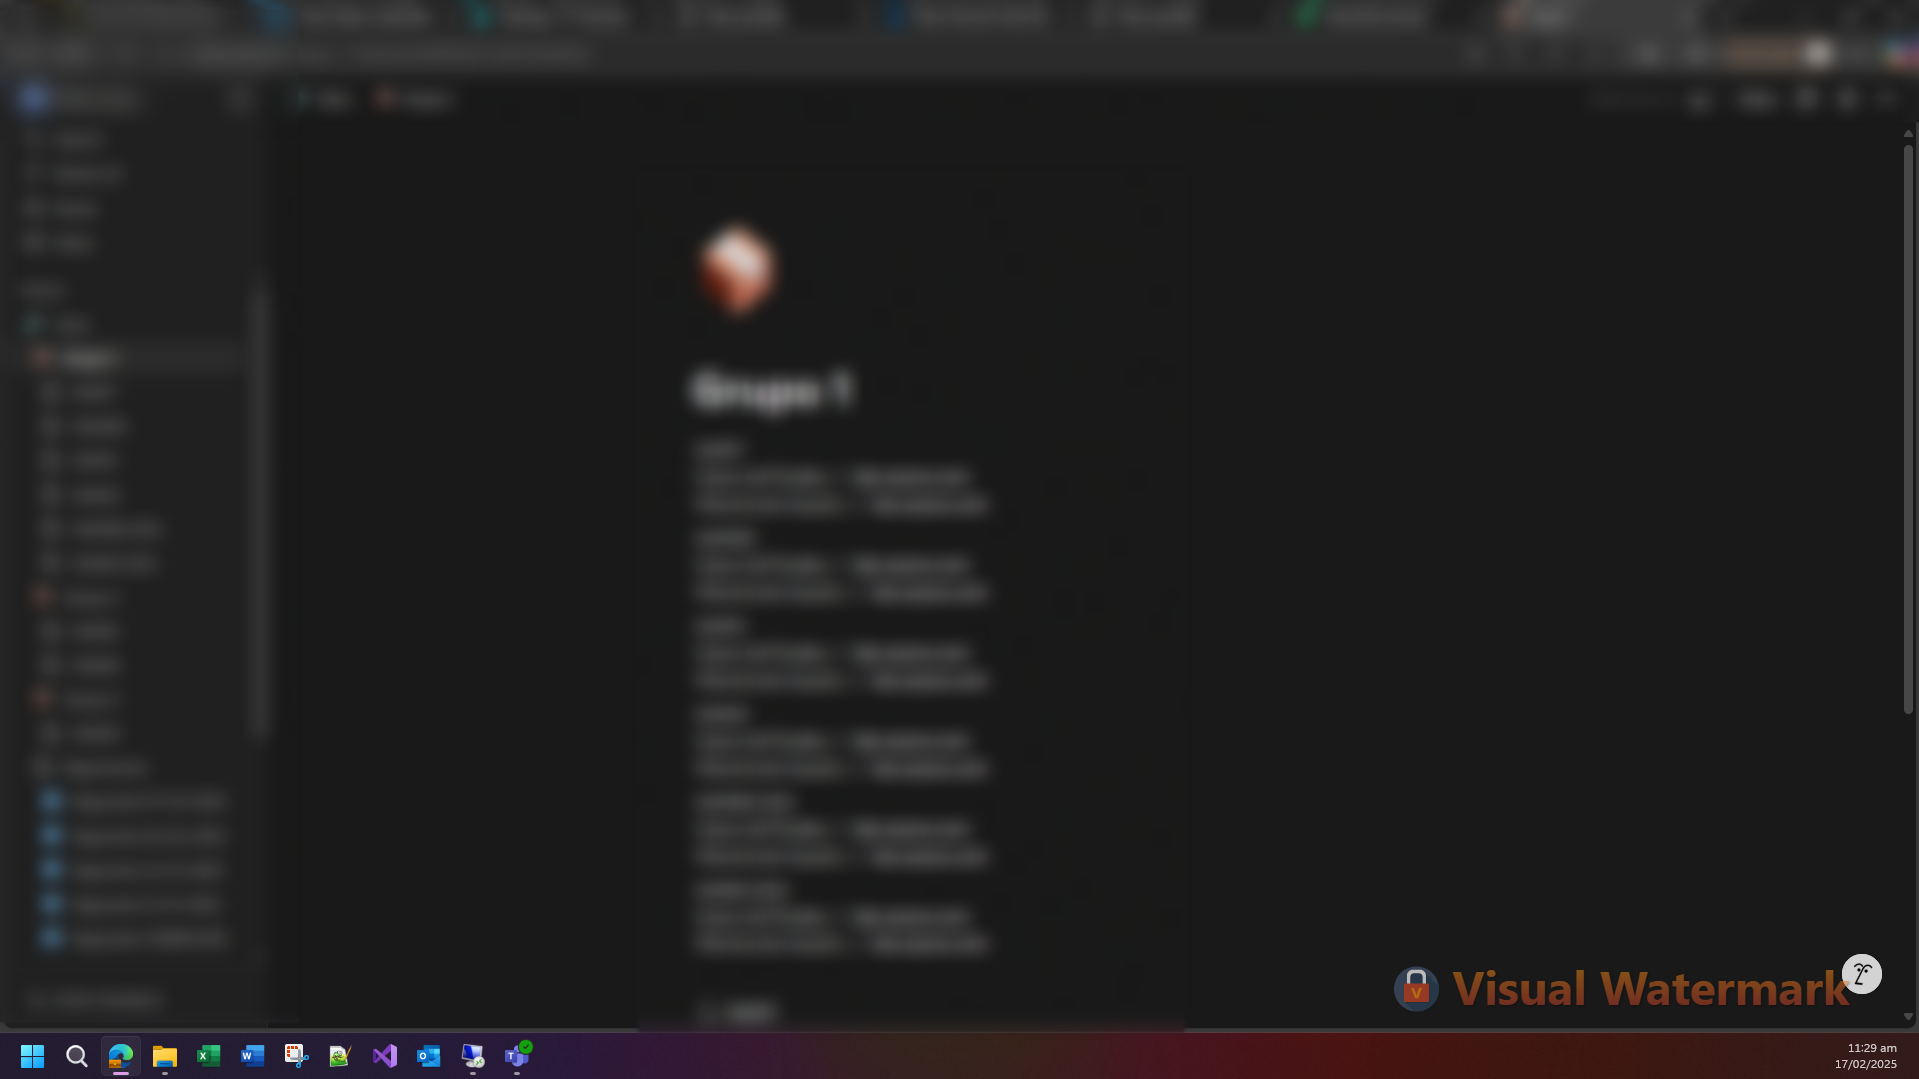
\includegraphics[width=14cm]{images/evidenciatareasrealizadas/notion.png}
      \caption{Seguimiento de evidencias en Notion}
    \end{figure}
    \item \textbf{Fotografías:}
    \begin{figure}[H]
      \centering
      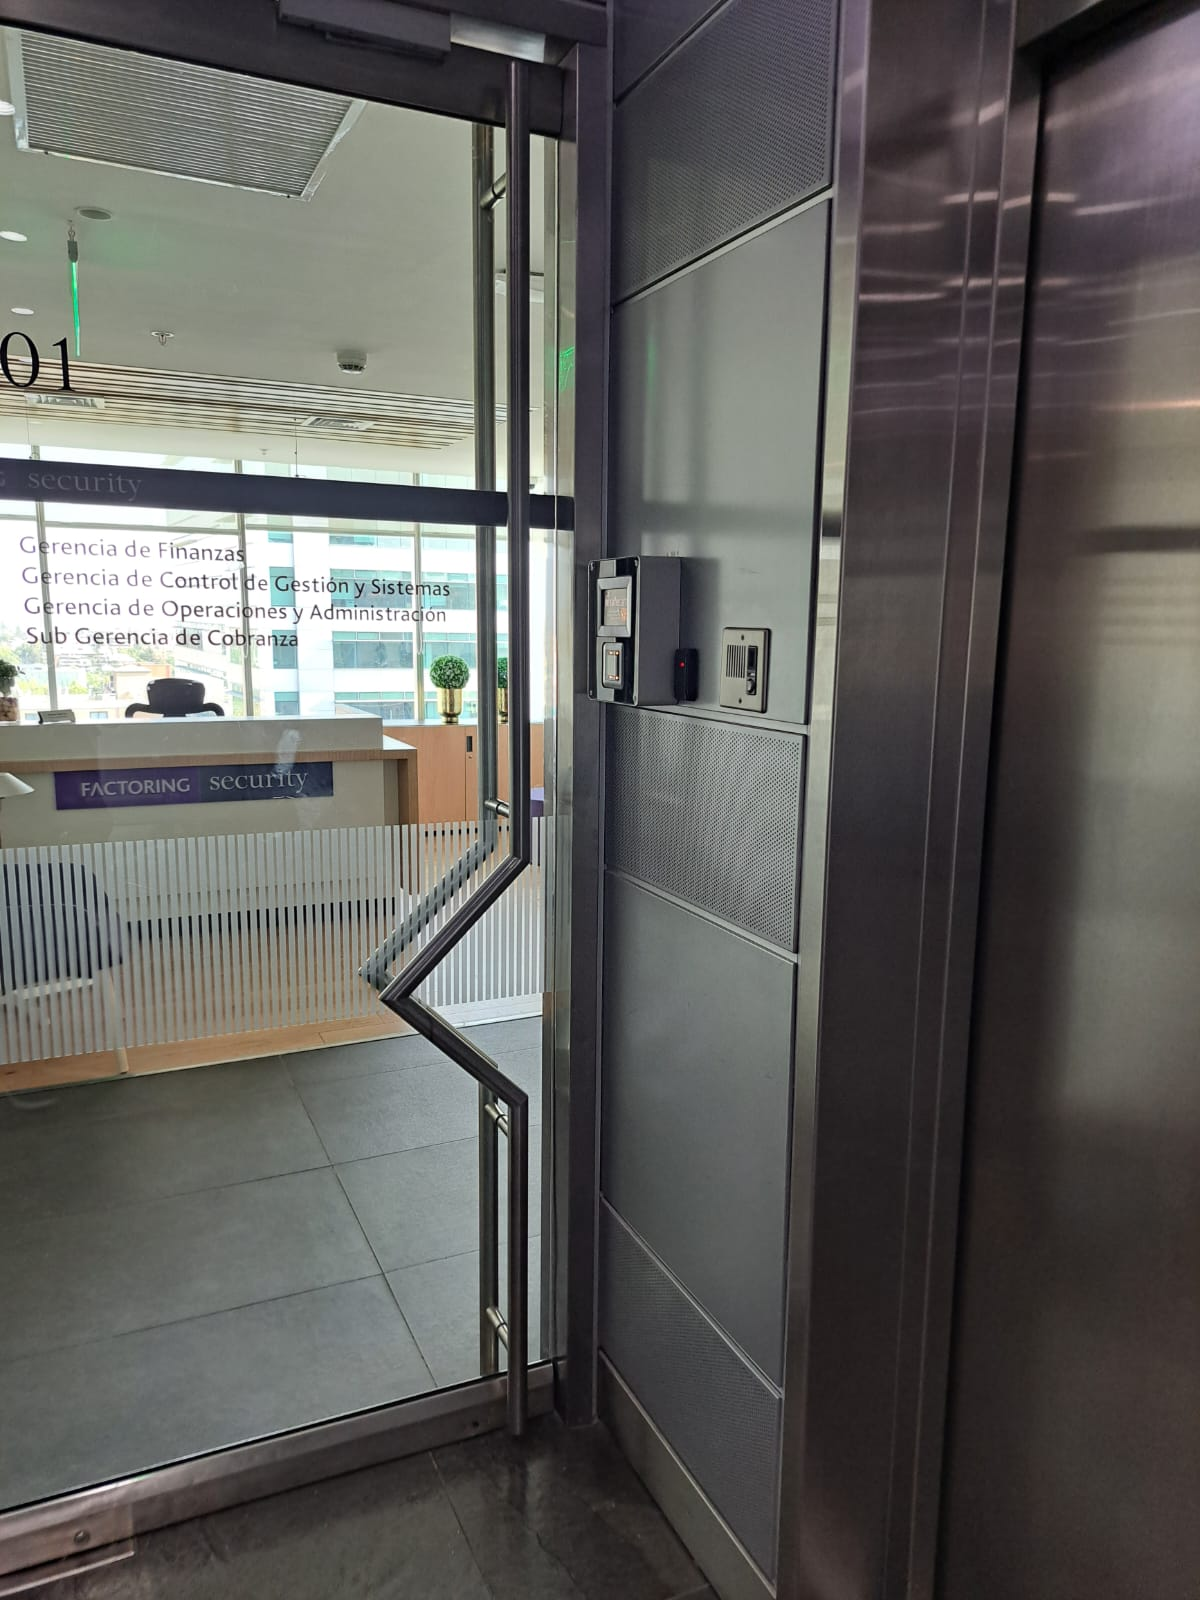
\includegraphics[width=14cm]{images/fotografias/oficina-2.jpeg}
      \caption{Oficina de Factoring Security}
    \end{figure}
    \begin{figure}[H]
      \centering
      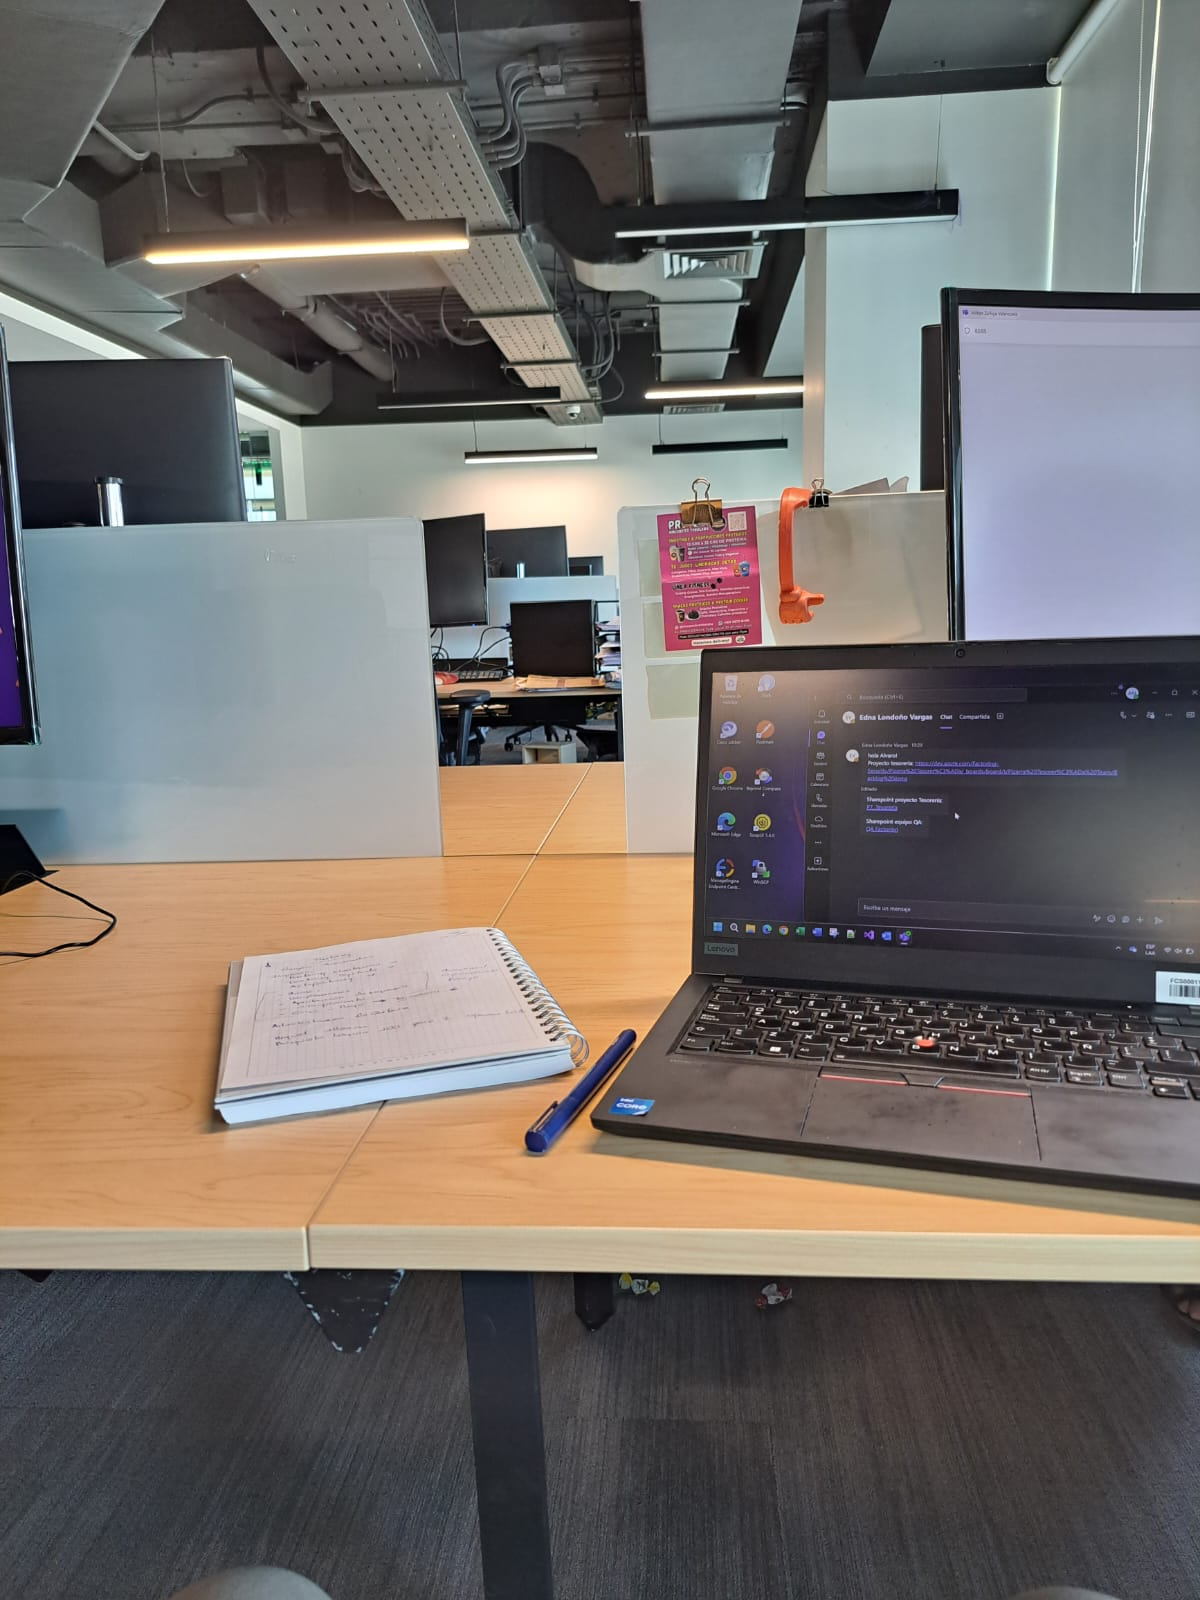
\includegraphics[width=14cm]{images/fotografias/oficina-1.jpeg}
      \caption{Área de trabajo en Factoring Security}
    \end{figure}
    \item \textbf{Pantallas:}
    \begin{figure}[H]
      \centering
      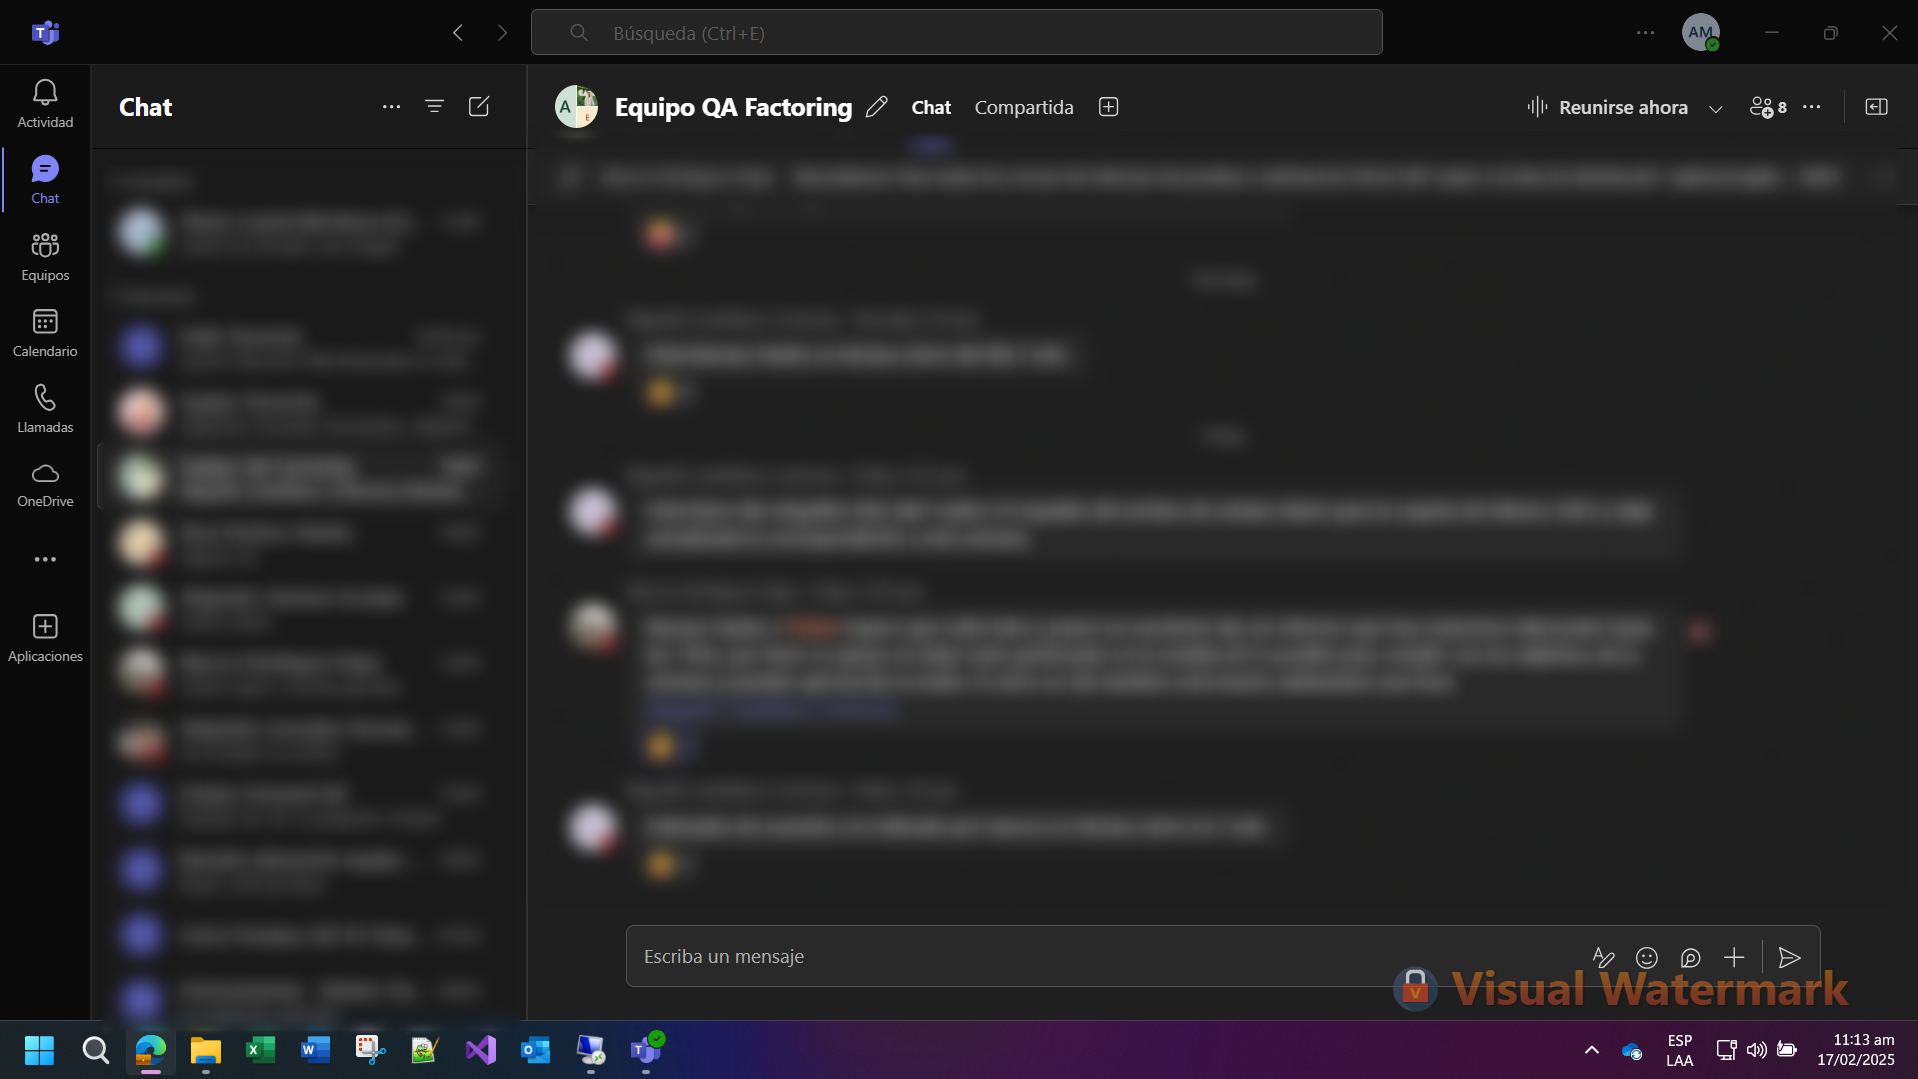
\includegraphics[width=14cm]{images/pantallas/teams.png}
      \caption{Plataforma Microsoft Teams utilizada para reuniones y comunicación interna}
    \end{figure}
    \begin{figure}[H]
      \centering
      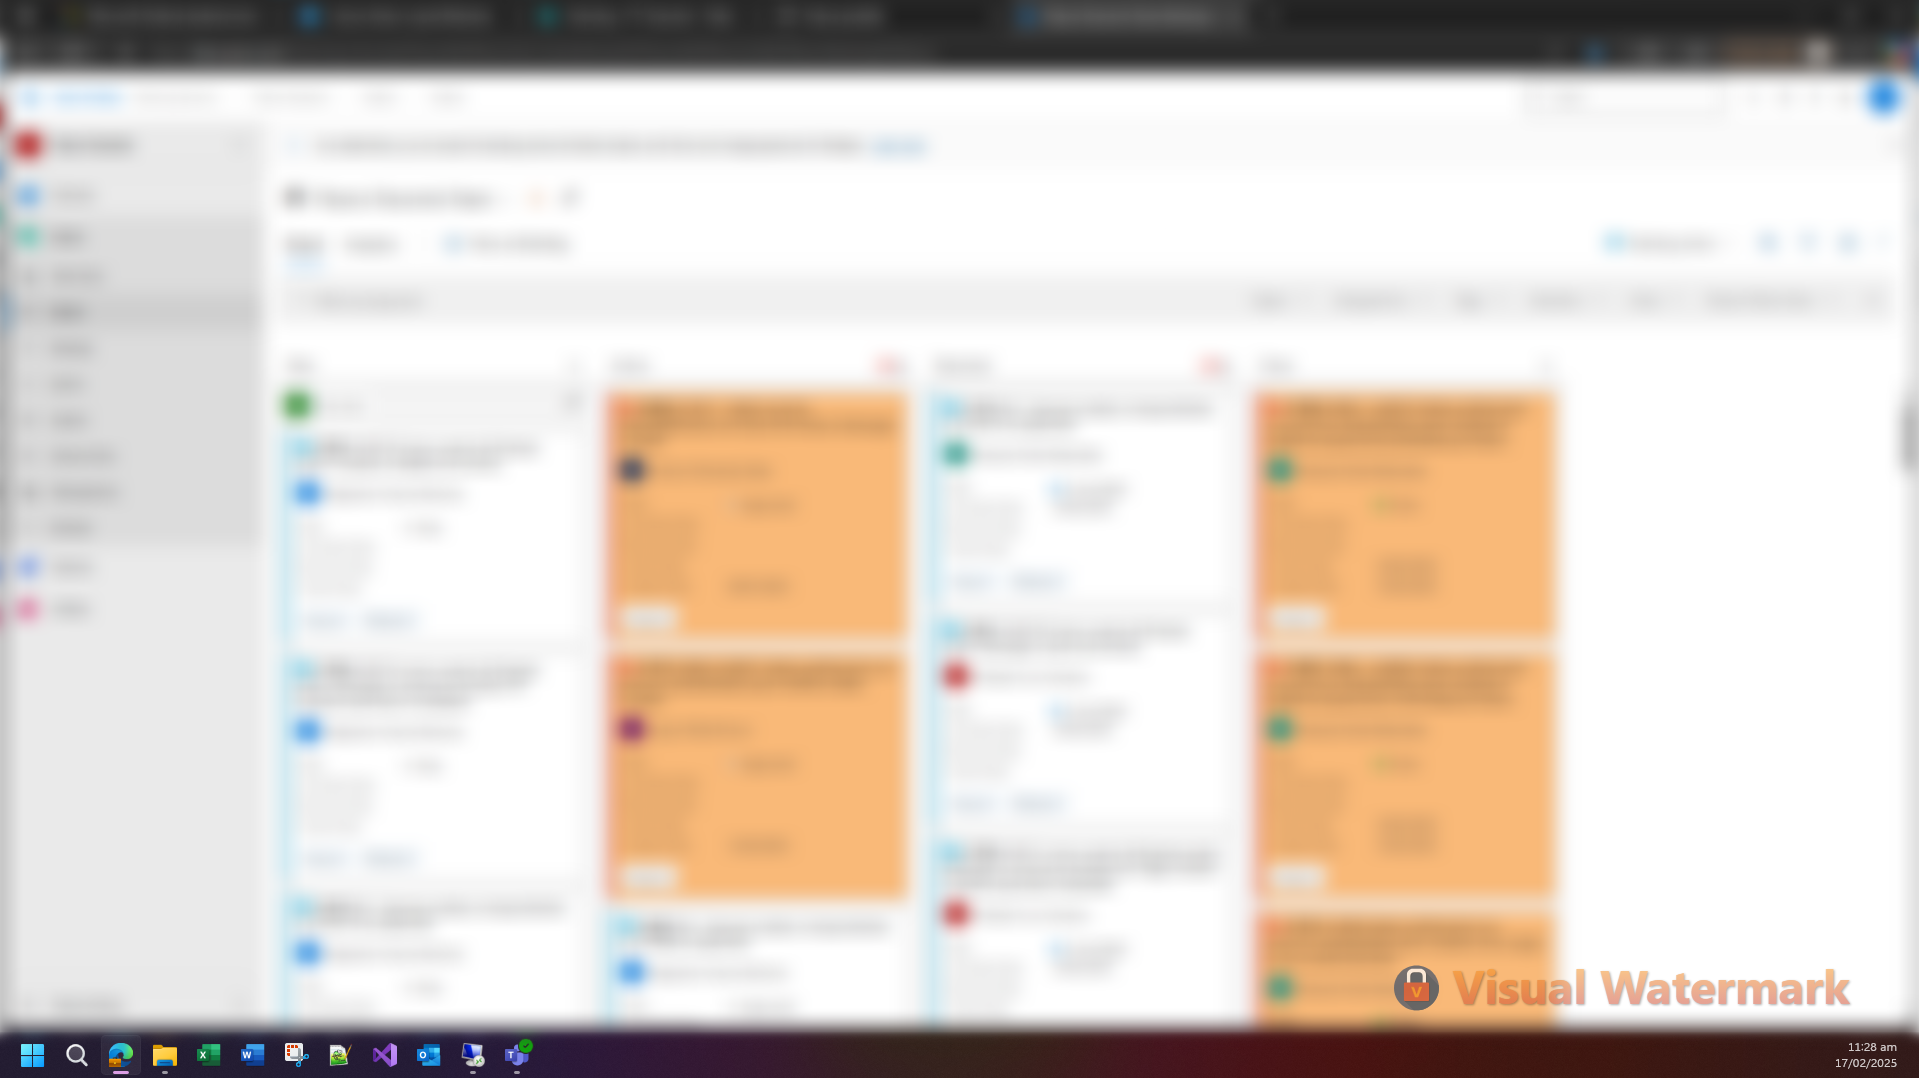
\includegraphics[width=14cm]{images/pantallas/azure-board.png}
      \caption{Plataforma Microsoft Azure DevOps para gestión de tareas}
    \end{figure}
    \begin{figure}[H]
      \centering
      
\includegraphics[width=14cm]{images/pantallas/azure-backlogs.png}
      \caption{Plataforma Microsoft Azure DevOps para seguimiento de tareas y reporte de defectos}
    \end{figure}
    \begin{figure}[H]
      \centering
      
\includegraphics[width=14cm]{images/pantallas/centralizacion-de-sistemas.png}
      \caption{Centralización de sistemas en el proyecto de cambio de core}
    \end{figure}
    \begin{figure}[H]
      \centering
      
\includegraphics[width=14cm]{images/pantallas/sistema-factoring.png}
      \caption{Sistema de factoring para gestión de operaciones financieras}
    \end{figure}
    \begin{figure}[H]
      \centering
      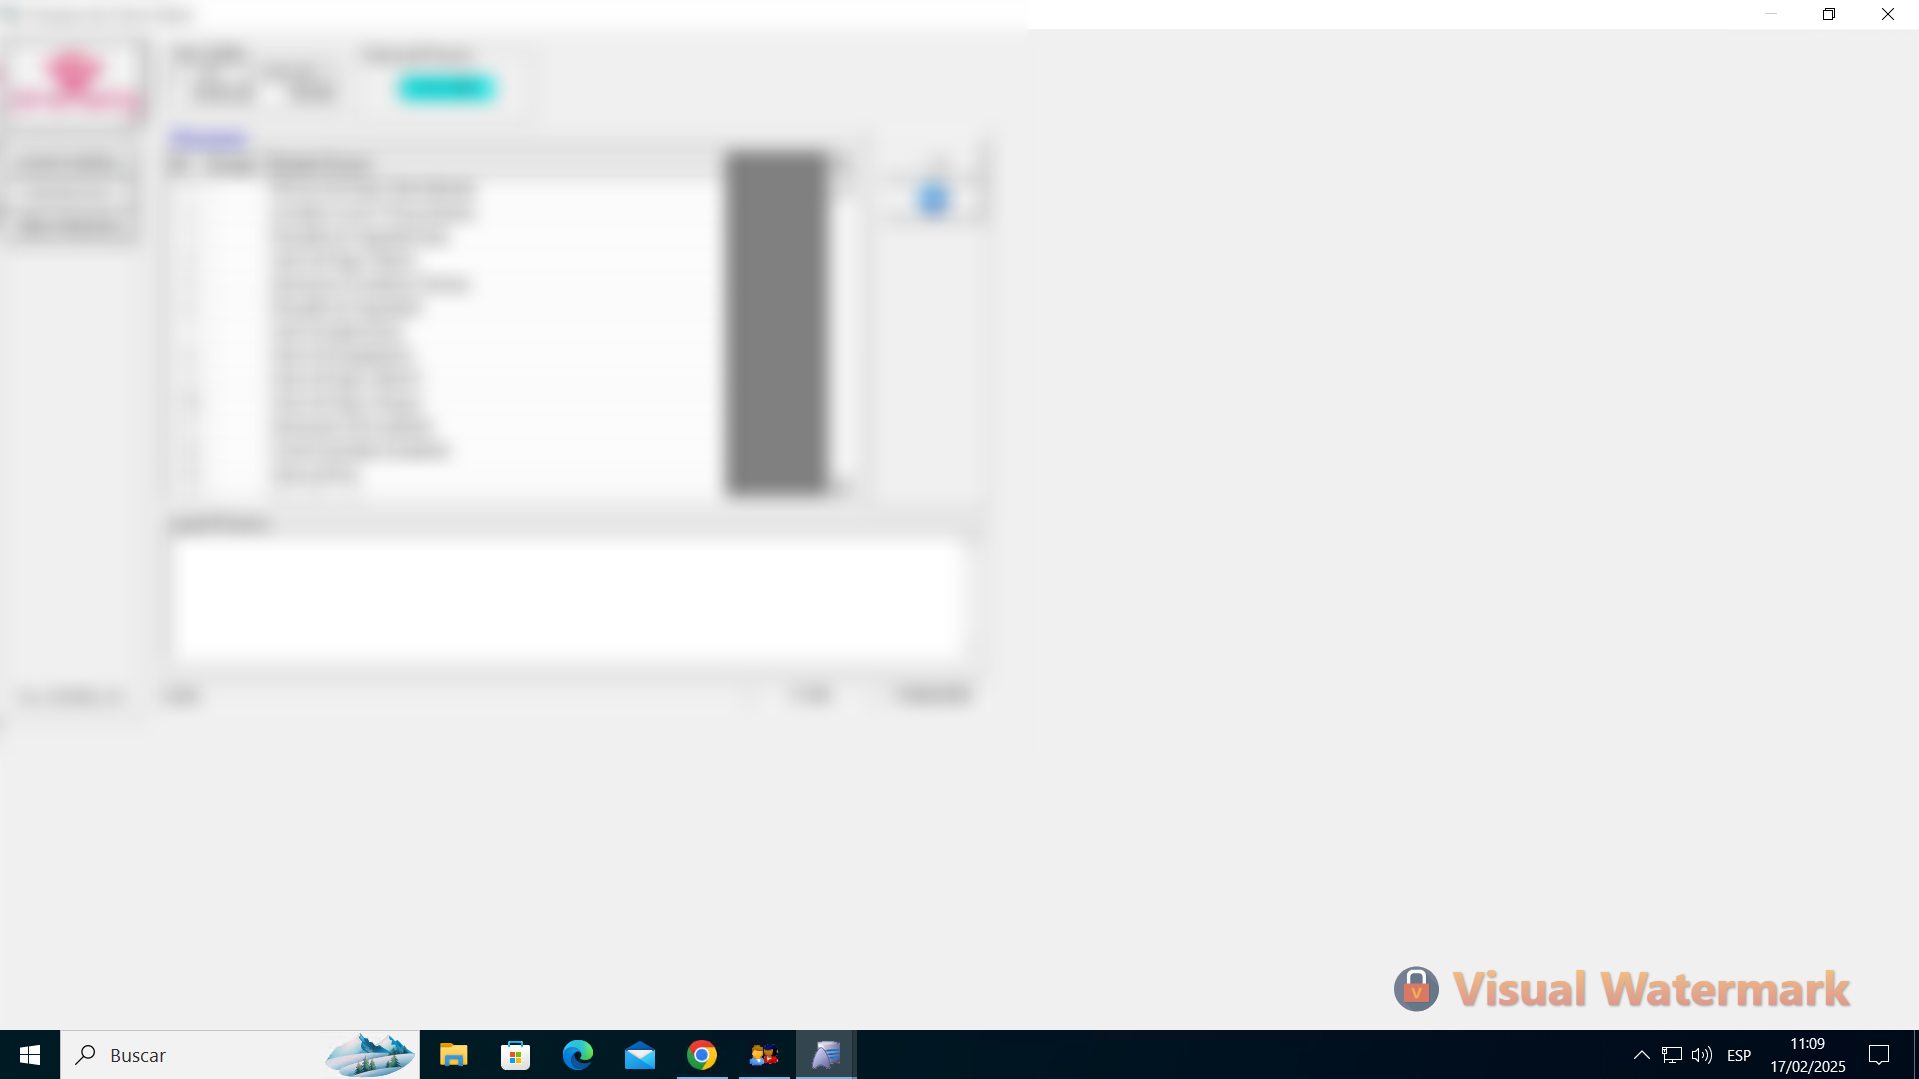
\includegraphics[width=14cm]{images/pantallas/mantencion-procesos.png}
      \caption{Sistema de mantención de procesos}
    \end{figure}
    \begin{figure}[H]
      \centering
      
\includegraphics[width=14cm]{images/pantallas/mantencion-dolar.png}
      \caption{Sistema de mantención de valores del dólar}
    \end{figure}
    \begin{figure}[H]
      \centering
      
\includegraphics[width=14cm]{images/pantallas/nuevo-curse.png}
      \caption{Sistema de gestión nuevos negocios}
    \end{figure}
    \begin{figure}[H]
      \centering
      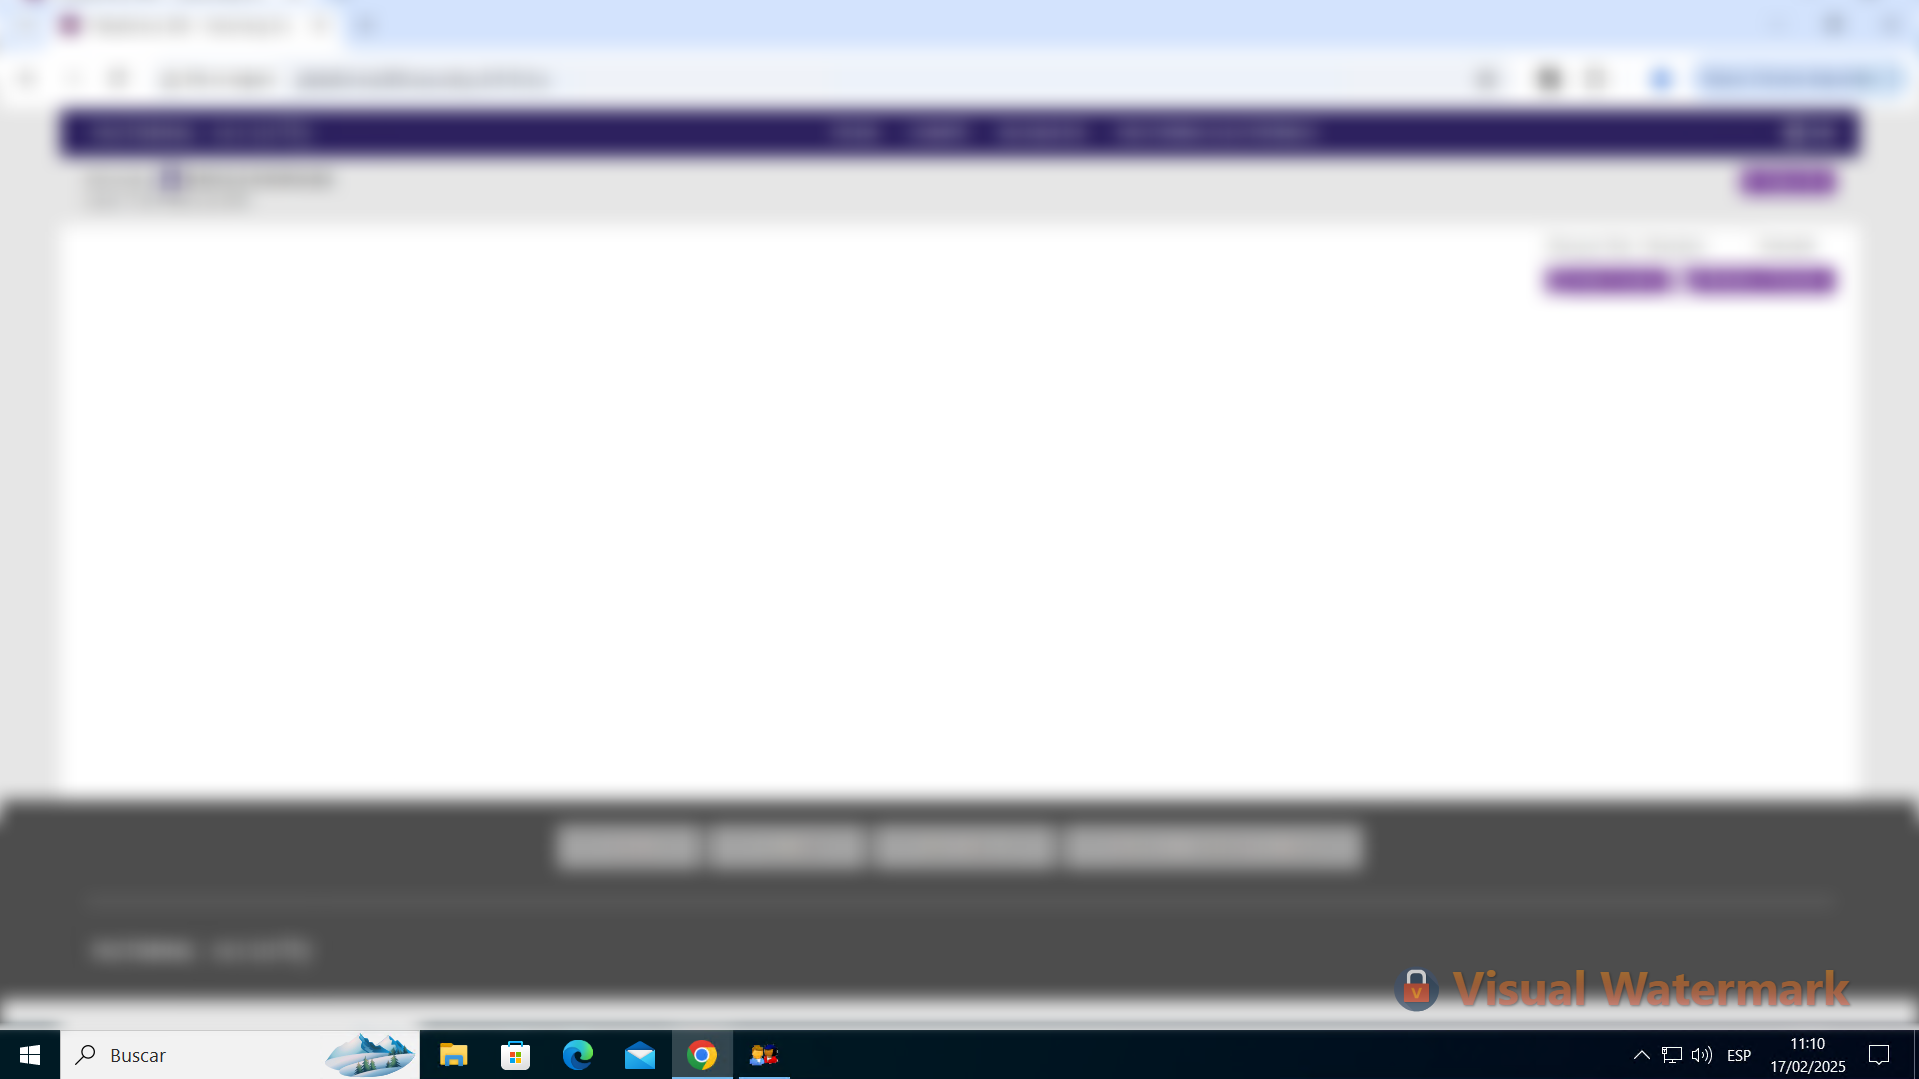
\includegraphics[width=14cm]{images/pantallas/p360.png}
      \caption{Plataforma 360 para centralización de información}
    \end{figure}
    \begin{figure}[H]
      \centering
      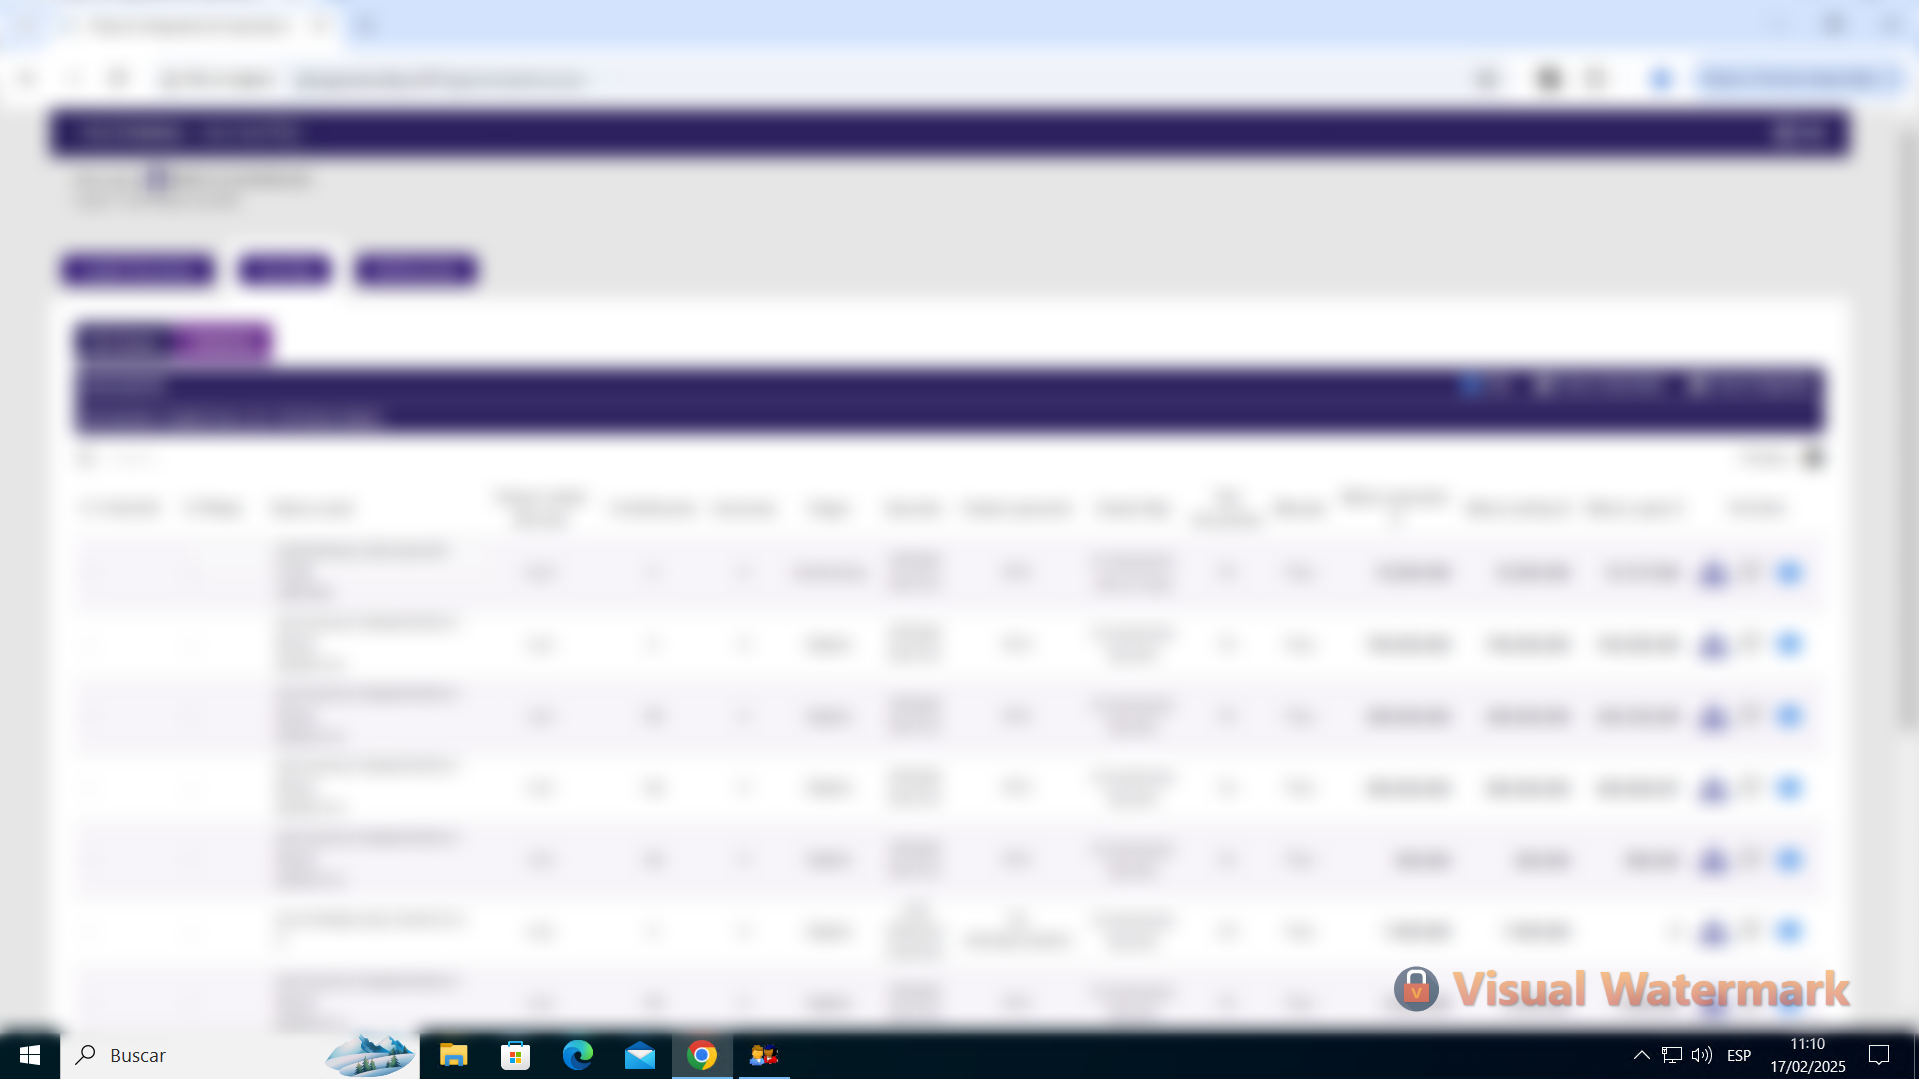
\includegraphics[width=14cm]{images/pantallas/pia.png}
      \caption{Pizarra Integrada de Aprobación (PIA) para validación de operaciones}
    \end{figure}
    \begin{figure}[H]
      \centering
      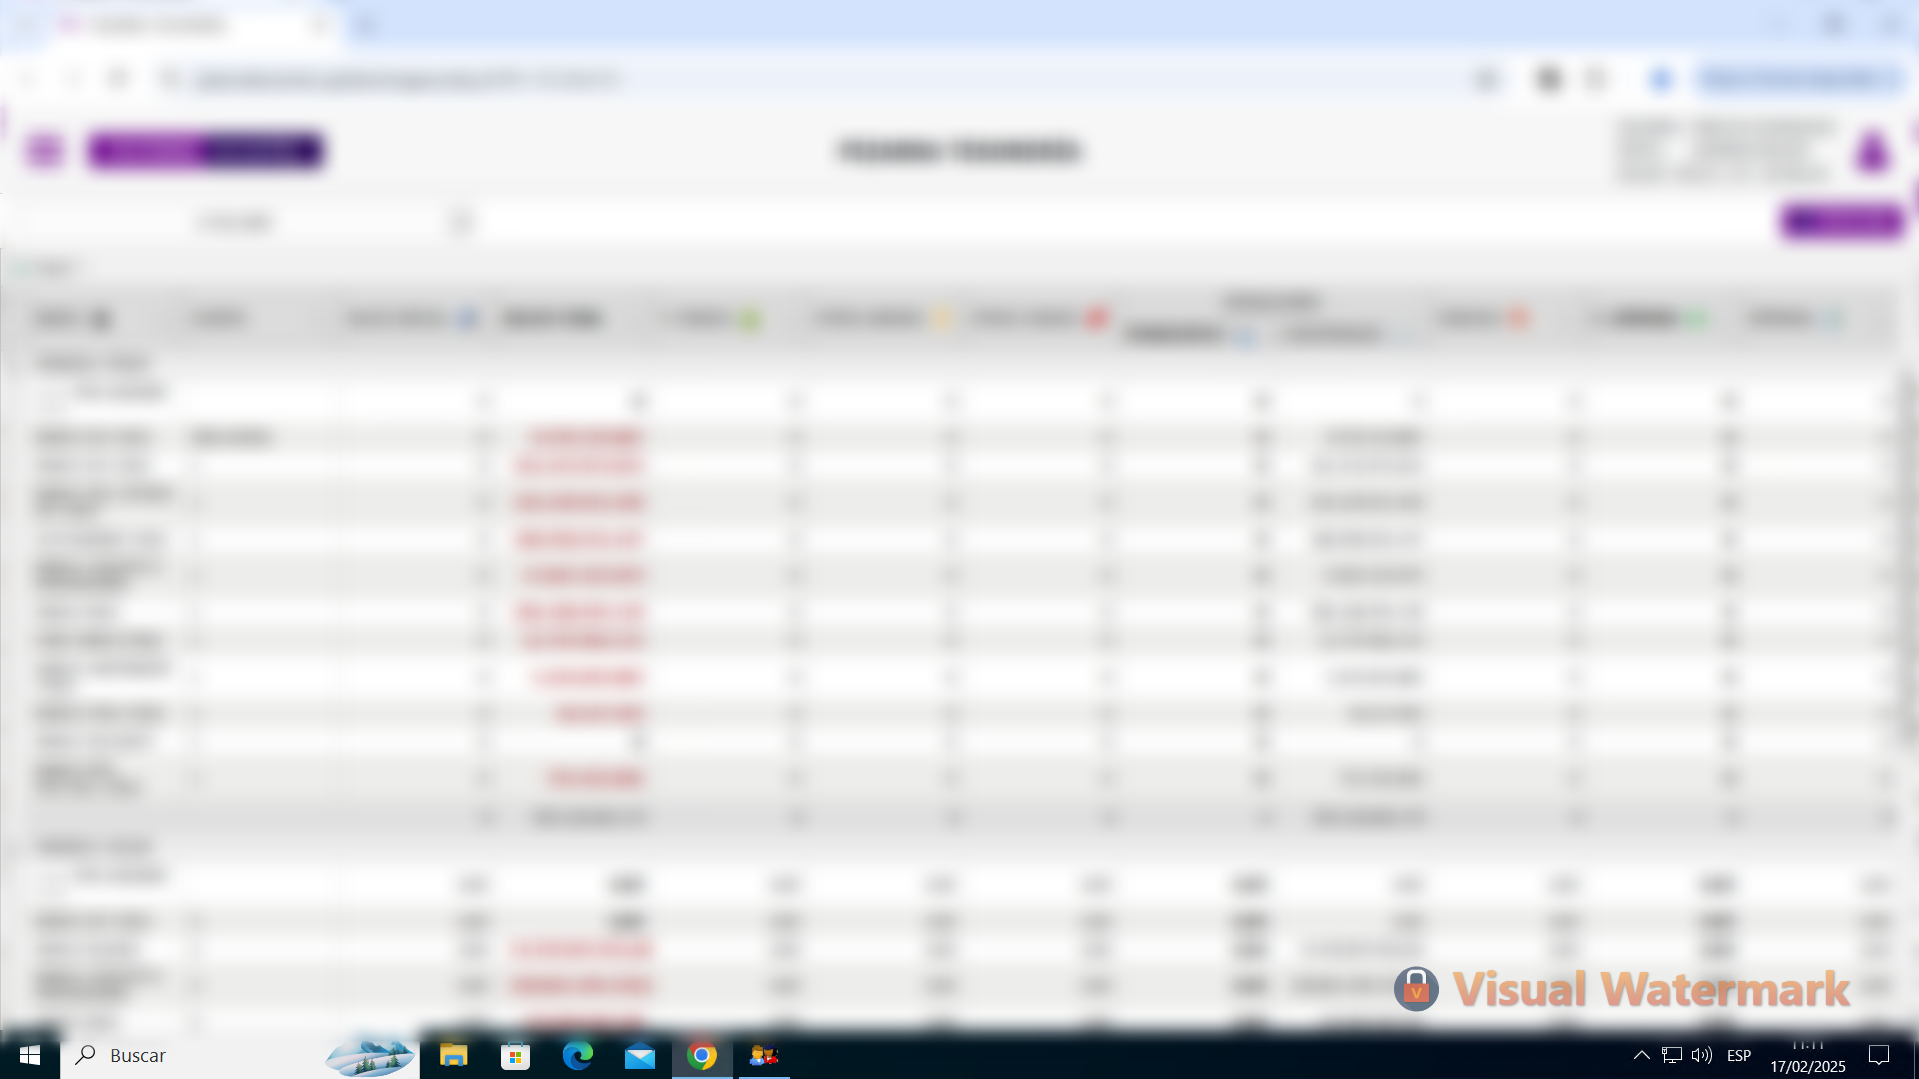
\includegraphics[width=14cm]{images/pantallas/pizarra-tesoreria.png}
      \caption{Pizarra de Tesorería para control de operaciones financieras}
    \end{figure}
    \item \textbf{Manuales y documentos:}
    \begin{figure}[H]
      \centering
      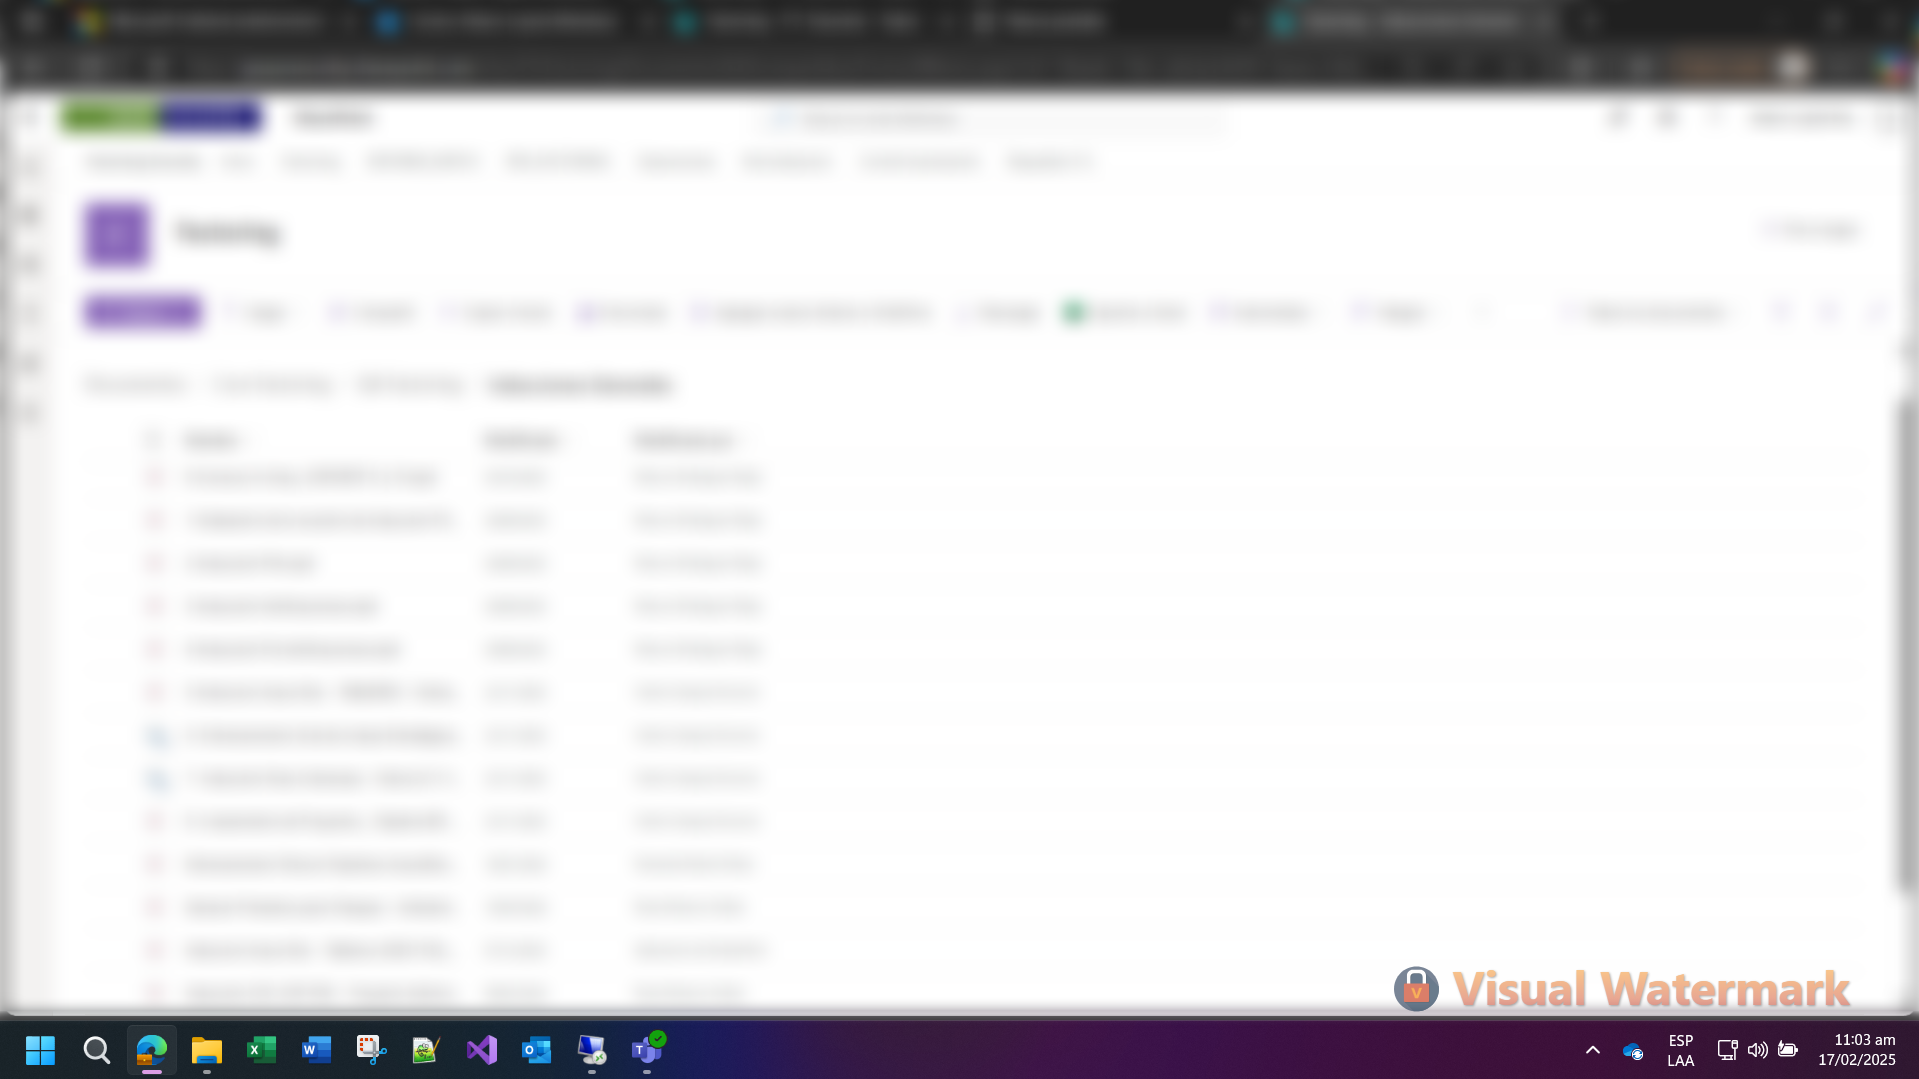
\includegraphics[width=14cm]{images/manualesydocumentos/sharepoint.png}
      \caption{Sharepoint con documentos y manuales de la empresa}
    \end{figure}
    \item \textbf{Bitácoras:}
    Documento aparte, debo adjuntarlo una vez terminado.
\end{itemize}
\end{document}
